\documentclass{article}

\usepackage[utf8]{inputenc}
\usepackage[brazil]{babel}
\usepackage{amsmath}
\usepackage{amsfonts}
\usepackage[section]{placeins}
\usepackage{booktabs}
\usepackage{multirow}
\usepackage{listings}
\usepackage{booktabs}
\usepackage[title]{appendix}

\usepackage{caption}

\usepackage{hanging}
\usepackage{graphicx}

\usepackage{natbib}

% Commands --------------------------------------------------------------------

\newcommand\indep{\protect\mathpalette{\protect\independenT}{\perp}}
\def\independenT#1#2{\mathrel{\rlap{$#1#2$}\mkern2mu{#1#2}}}

\setlength{\parskip}{0.5em}

\def\arraystretch{1.5}

% Document basics -------------------------------------------------------------

\title{Métodos Numéricos - Lista 03}
\author{Samuel de S. Barbosa}
\date{Junho, 2018}

\begin{document}

\maketitle

\section*{}

Nesta lista vamos solucionar o modelo de \textit{Real Business Cycles} (RBC) usando
métodos de projeção.


\subsubsection*{Preferências}

$$ U(c) = \mathbb{E}_0 \sum_{t=0}^{\infty} \beta^t u(c_t) $$

$$ u(c_t) = \frac{c^{1-\mu}-1}{1-\mu}$$
$$\mu = 1/(1+r)$$

\subsubsection*{Tecnologia}

$$Y_t = z_t F(K_t, N_t) = z_t K_t^\alpha N_t^{1-\alpha}$$

$$ \log z_t = \rho \log z_{t-1} + \epsilon_t $$

$$ \varepsilon_t \sim N(0, \sigma^2) $$

\subsubsection*{Calibração}

$$\beta = 0.987, \,\,\,\,\, \mu=2, \,\,\,\,\,  \alpha=0.3, \,\,\,\,\,  \delta=0.012, \,\,\,\,\,  \rho=0.95, \,\,\,\,\, \sigma=0.007$$

\newpage


% ----------------------------------------------------------------------------------------------------------------------------------------
\subsubsection*{1. Polinômios de Chebyshev e \textit{collocation points}}

Os métodos de projeção são métodos gerais utilizados para obter soluções
aproximadas para equações funcionais. Com os métodos de projeção,
encontramos uma função (e não apenas uma sequência de valores, tal como
nos métodos de iteração da função valor) que resolve uma dada equação funcional.

No problema em questão, a equação funcional a ser resolvida é a Equação de Euler:

\begin{equation}
\begin{aligned}
u^{\prime}(c) & = & & \beta  \mathbb{E} [ \frac{\partial}{\partial k^{\prime}} V(k^{\prime},z^{\prime})] \\
      & = & & \beta  \mathbb{E} [u^{\prime}(c^{\prime}) (\alpha z k^{\alpha-1} + 1 - \delta)].
\end{aligned}
\end{equation}

O método de projeção que iremos aplicar será o dos polinômios de Chebyshev,
em conjunto com o uso de \textit{collocation points}. A função que obteremos
séra uma combinação convexa de polinômios, avaliada em pontos de colocação
tais que estes polinômios serão ortogonais entre si.

Um polinômio de Chebyshev de grau $p$ é dado por $T_p(x) = cos(p cos^{-1}(x))$.
Os pontos de colocação utilizados serão as $(p+1)$ raízes de um polinômio de Chebyshev
de grau $p+1$: 

$$ z_i = -cos\left(\frac{2i-1}{2p}\pi\right) $$

A aproximação da função política do consumo que resolve a Equação de Euler será
obtida por 

$$ \hat{C}(\gamma,K) = \sum_{j=0}^p \gamma_j T_j(K)$$

A figura a seguir mostra os resultados obtidos através da aplicação deste método:

\begin{figure}[h!]
  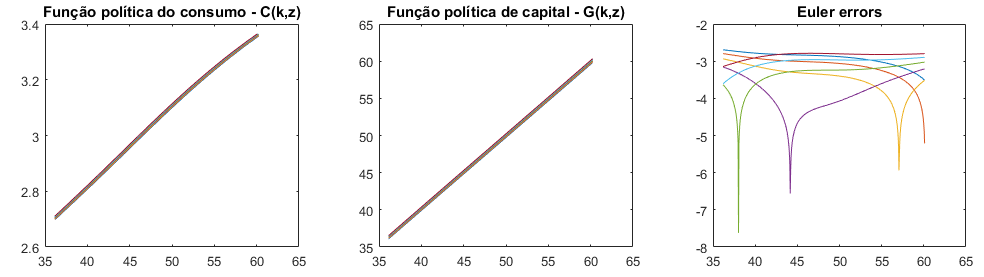
\includegraphics[width=\linewidth]{graf1.png}
\end{figure}

Observação: a solução implementada é muito sensível ao chute inicial 
de $\gamma$ (pesos atribuídos a cada polinômio). Para obter a solução
final, dependendo dos graus de polinômios utilizados, eventualmente 
foi necessário executar o código várias vezes com chutes iniciais
aleatórios até obter convergência. 

\end{document}
